\documentclass[12pt,a4paper,CJK]{beamer}
\usepackage[utf8]{inputenc}
\usepackage{amsmath}
\usepackage{amsfonts}
\usepackage{amssymb}
\usepackage{CJK}										% 支持中文
\usepackage{color}						% 给文字,表格和图形上色(68种)
\usepackage{xcolor}									% color包的扩展

%================================主题设置=============================%
\usetheme{Boadilla}									% PPT主题
\usefonttheme{serif} 
\useinnertheme{umbcboxes}


%================================具体设置=============================%
\setbeamercolor{umbcboxes}{bg=violet!12,fg=black}
\setbeamertemplate{navigation symbols}{}				% 取消引导
\hypersetup{colorlinks,citecolor = blue, linkcolor=blue}
\DeclareMathOperator*{\argmax}{arg\,max}
	
%============================++++++++++++============================%
\author{hjy}
\title{KFDA}
\institute{TongJi University}
\date{\today}	
%============================++++++++++++============================%	




\begin{document}
\begin{CJK*}{UTF8}{gkai}
%----------- titlepage ----------------------------------------------%
\begin{frame} 				
	\titlepage 
\end{frame}
	
%----------- outline ------------------------------------------------%
\begin{frame}
	\frametitle{目录}
	\tableofcontents
\end{frame}
  
%--------------------------------------------------------------------%
\section{Fisher线性判别分析(C类)}
\begin{frame}{\secname}
	\begin{itemize}
	\item 核心思想(详情参见课件PatternClassification\_{}8.ppt)\\
		选择使得 Fisher准则函数达到极值的矢量作为最佳投影方向$\overrightarrow{W}$,从而使得样本在该方向上投影后,达到最大的类间离散度$S_b$和最小的类内离散度$S_w$.
	\item 表达式\\
		\begin{displaybox}{90mm}
		\[ 			
 			\vec{W^*} = 
 			\argmax_{\vec{W}} J(\vec{W})=
 			\argmax_{\vec{W}} \Bigl(
 			\frac{\vec{W}^T S_b \vec{W}}{\vec{W}^T S_w \vec{W}}
 			\Bigr)
 		\]
 			
 		\[
 			S_b = \sum_{i=1}^{c} N_i(\vec{\upsilon_i}-\upsilon)^T(\vec{\upsilon_i}-\upsilon)
 		\]
 		
 		\[
 			S_w = \sum_{i=1}^{c} \sum_{j=1}^{N_i}(\vec{X_i^j}-\vec{\upsilon_i})^T(\vec{X_i^j}-\vec{\upsilon_i})
 		\]
 		
		\end{displaybox}
	\end{itemize}
\end{frame}


%--------------------------------------------------------------------%
\section{核函数}
\subsection{定义}
\begin{frame}{\subsecname}
	\begin{itemize}
	\item 核函数\\
		设$x,z \in X, X$属于 $R(n)$空间,非线性映射函数 $\phi$实现输入空间 $X$到特征空间 $F$的映射,其中 $F$属于 $R(m), n<<m$。根据核函数技术有:
		\begin{displaybox}{90mm}
		\[ 
			\kappa(\vec{X},\vec{Z}) =\langle \phi(\vec{X}),\phi(\vec{Z})\rangle
		\]
		\end{displaybox}
		其中: $\langle, \rangle$ 为内积, $\kappa(x,z)$为核函数。\\
		从上式可以看出,核函数\textcolor{red}{将 $m$维高维特征空间的内积运算转化为 $n$维低维输入空间的核函数计算},巧妙地解决了在高维特征空间中计算中可能出现的“维数灾难”等问题,从而为在高维特征空间中解决复杂的分类或回归问题奠定了理论基础。
	\end{itemize}
\end{frame}


%--------------------------------------------------------------------%
\subsection{性质}
\begin{frame}{\subsecname}
接受低维空间的输入值$\vec{X}$和$\vec{Z}$,却能算出高维空间的内积值$\langle \phi(\vec{X}),\phi(\vec{Z})\rangle$.
\begin{columns}
  \begin{column}{.50\textwidth}
    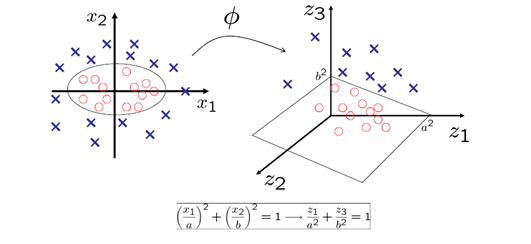
\includegraphics[scale=0.35]{figs/projection.png}
    \smallskip

    特征映射: \\
  	\begin{onlinebox}{55mm} 
  		$\displaystyle  
  			\phi(x_1,x_2)=(x_1^2,\sqrt{2}x_1x_2,x_2^2)
  		$
  	\end{onlinebox}
  \end{column}
\pause
  \begin{column}{.50\textwidth}
  \begin{definition}
  		\[
  			\vec{X} =(x_1,x_2) \quad \vec{Z} ={z_1,z_2} 
  		\]\[
			\kappa(\vec{X},\vec{Z}) =\langle \phi(\vec{X}),\phi(\vec{Z})\rangle	
		\]\[\qquad =(\vec{X}\cdot\vec{Z})^2
		\]

  \end{definition}  
    \begin{displaybox}{64mm}
		$\kappa(\vec{X},\vec{X}) =(\vec{X}\cdot\vec{Z})^2$\\
		$=(x_1z_1+x_2z_2)^2$\\
		$=(x_1^2,\sqrt{2}x_1x_2,x_2^2)*(z_1^2,\sqrt{2}z_1z_2,z_2^2)$\\
		$=\langle \phi(\vec{X}),\phi(\vec{Z})\rangle	$
	\end{displaybox}
  
  \end{column}
\end{columns}
\end{frame}


%--------------------------------------------------------------------%
\section{核Fisher判别法}
\subsection{定义}
\begin{frame}{\subsecname}
	基于核的 Fisher线性鉴别分析方法能够在原始输入空间中抽取非线性(在高维空间呈线性)最佳鉴别特征.
	对于一个数据集 $\chi$和一个特征映射函数 $\phi$,在 F空间类间散布矩阵 $S_b^\phi$和类内散布矩阵$S_w^\phi$ 可以被定义为:
	\begin{displaybox}{90mm}
 		\[
 		S_b^\phi=\sum_{i=1}^{c}N_i(\vec{\upsilon_i}^\phi-\upsilon^\phi)(\vec{\upsilon_i}^\phi-\upsilon^\phi)^T 		
 		\]\[
 			S_w^\phi = \sum_{i=1}^{c} \sum_{j=1}^{N_i}(\phi(\vec{X_i^j})-\vec{\upsilon_i})(\phi(\vec{X_i^j})-\vec{\upsilon_i})^T 		\]
	\end{displaybox}
	在特征空间 F中利用最大化线性准则函数获取最优投影方向:
	\begin{displaybox}{90mm}
 		\[ 			
 			\vec{V^*} = 
 			\argmax_{\vec{V}} J(\vec{V})=
 			\argmax_{\vec{V}} \Bigl(
 			\frac{\vec{V}^T S_b^\phi \vec{V}}{\vec{V}^T S_w^\phi \vec{V}}
 			\Bigr)
 		\]
	\end{displaybox}
\end{frame}

%--------------------------------------------------------------------%
\subsection{推理过程1}
\begin{frame}{\subsecname}
易知$\vec{V} \in F$, 即 $\vec{V}$一定在由 $\phi(X_i^j)$所伸展的空间中,因此它
可以表示为:
	\begin{displaybox}{123mm}
 		\[ 			
 			\vec{V} = \sum_{i=1}^{c} \sum_{j=1}^{N_i}
 			w_i^j\vec{\phi(X_i^j)} = \phi(X)^T\vec{W}
 		\]
注: 		\\
 		$
 			\vec{W} = (w_1^1,\cdots,w_1^{N_1},\ldots,w_c^1,\cdots,w_c^{N_c})^T  \qquad \textcolor{red}{\sum_{i=1}^{c}N_i*1}
 		$\\$
 			\phi(X)=(\vec{\phi(X_1^1)},\cdots,\vec{\phi(X_1^{N_1})},\ldots,\vec{\phi(X_c^1)},\cdots,\vec{\phi(X_c^{N_c})})^T  \: \textcolor{red}{\sum_{i=1}^{c}N_i*m}
 		$
	\end{displaybox}
带入到上式得到:
	\begin{displaybox}{90mm}
 		\[ 			
 			\vec{V}^T S_b^\phi \vec{V} = \vec{W}^T\lbrace \phi(X)^TS_b^\phi\phi(X)\rbrace \vec{W}
 		\]\[ 			
 			\vec{V}^T S_w^\phi \vec{V} = \vec{W}^T\lbrace \phi(X)^TS_w^\phi\phi(X)\rbrace \vec{W}
 		\]
	\end{displaybox}
	
\end{frame}


%--------------------------------------------------------------------%
\subsection{推理过程2}
\begin{frame}{\subsecname}
上式$\lbrace \rbrace$中分别用$K_b$和$K_w$表示[$K_b$和$K_w$都是\textcolor{red}{$\sum_{i=1}^{c}N_i*\sum_{i=1}^{c}N_i$}],则问题转变为:
	\begin{displaybox}{90mm}
		\[ 			
 			\vec{W^*} = 
 			\argmax_{\vec{W}} J(\vec{W})=
 			\argmax_{\vec{W}} \Bigl(
 			\frac{\vec{W}^T K_b \vec{W}}{\vec{W}^T K_w \vec{W}}
 			\Bigr)
 		\]
 	\end{displaybox}
由广义的瑞利商得:
	\begin{displaybox}{90mm}
		$\vec{W^*}$为$K_w^{-1}K_b$的$\sum_{i=1}^{c}N_i$个特征向量中的一个.
		\textcolor{red}{$\vec{W^*}$为$\sum_{i=1}^{c}N_i*1$维向量.}	
 	\end{displaybox}
\end{frame}


%--------------------------------------------------------------------%
\subsection{推理结果}
\begin{frame}{\subsecname}
	\begin{displaybox}{90mm}
		\[ 			
 			W = (\vec{W_1},\cdots,\vec{W_m})			
 		\]
 		注:\\
 		$\vec{W_i}(1 \leq i \leq m)$为$K_w^{-1}K_b$的m个最大的特征向量 		
 	\end{displaybox}
对于任何一个输入矢量 $\vec{X}$,它的低维特征 $\vec{Y} = ( y_1,\cdots, y_m)$ 可以表示为:
	\begin{displaybox}{120mm}
		\[ 			
 			\vec{Y} = (\vec{W_1},\cdots,\vec{W_m})^T*
 			\]\[(\kappa(\vec{X_1^1},\vec{X}),\cdots,\kappa(\vec{X_1^{N_1}},\vec{X}),\ldots,\kappa(\vec{X_c^1},\vec{X}),\cdots,\kappa(\vec{X_c^{N_c}},\vec{X}))			
 		\]
 	\end{displaybox}



\end{frame}


%--------------------------------------------------------------------%
\subsection{疑惑}
\begin{frame}{\subsecname}
\begin{enumerate}
\item 推理结果:低维特征$\vec{Y}$代表了什么意义,为嘛它是m维(高维),而不是n维(低维)?\\
根据模式分类课件PatternClassification\_{}8.ppt第18,19页的推理可知:
\textcolor{green}{权重向量$\vec{W}$取的是$K_w^{-1}K_b$的最大特征值对应的特征向量.($\vec{W}$是$\sum_{i=1}^{c}N_i*1$的列向量)}\\
假定将训练样本集X(低维n)映射到F空间$\phi(X)$(高维m),并且用FDA方法求解出最优投影方向为$\vec{V}$,对于任何一个测试样本$\vec{T}$,它被映射成高维空间的$\phi(\vec{T})$,计算的标量$y=\vec{V}^T*\phi(\vec{T})$,根据y的具体数值区分$\phi(\vec{T})$属于哪一类.\cite{1}\\
\begin{displaybox}{115mm}
	核函数的定义: \quad $\kappa(\vec{X},\vec{W}) =\langle \phi(\vec{X}),\phi(\vec{W})\rangle$\\
	$y=\vec{V}^T*\phi(\vec{X})=\vec{W}^T*\phi(X)*\phi(\vec{T})$\\
	\qquad $=\vec{W}^T(\kappa(\vec{X_1^1},\vec{X}),\cdots,\kappa(\vec{X_1^{N_1}},\vec{X}),\ldots,\kappa(\vec{X_c^1},\vec{X}),\cdots,\kappa(\vec{X_c^{N_c}},\vec{X}))$
		
\end{displaybox}
\end{enumerate}





\end{frame}

%--------------------------------------------------------------------%
\section{参考}
\begin{frame}{\secname}

\nocite{*}
\bibliographystyle{unsrt}
\bibliography{ref/mybib}


\end{frame}
\end{CJK*}
\end{document}